\documentclass{tufte-handout}

%\geometry{showframe}% for debugging purposes -- displays the margins

\usepackage{amsmath}

% Set up the images/graphics package
\usepackage{asymptote} % for asymptote graphics
\usepackage{graphicx}
\setkeys{Gin}{width=\linewidth,totalheight=\textheight,keepaspectratio}
\graphicspath{{graphics/}}

\title{Algorithm Complexity}
\author[Warren MacEvoy]{Warren MacEvoy}
% \date{24 January 2009}  % if the \date{} command is left out, the current date will be used

% The following package makes prettier tables.  We're all about the bling!
\usepackage{booktabs}

\hypersetup{colorlinks} % Comment this line if you don't wish to have colored links
\usepackage{amsmath}
\usepackage{amssymb}
\usepackage{amsthm}
\usepackage{listings}
\usepackage{siunitx} % align decimals in tables
\usepackage{nth}     % 1st, 2nd, ...
\usepackage{microtype} % Improves character and word spacing
\usepackage{asymptote} % for asymptote graphics
\usepackage{ccicons}
\usepackage{lipsum} % Inserts dummy text
\usepackage{booktabs} % Better horizontal rules in tables
\usepackage{graphicx} % Needed to insert images into the document

% The units package provides nice, non-stacked fractions and better spacing
% for units.
\usepackage{units}

% The fancyvrb package lets us customize the formatting of verbatim
% environments.  We use a slightly smaller font.
\usepackage{fancyvrb}
\fvset{fontsize=\normalsize}

% Small sections of multiple columns
\usepackage{multicol}

% Provides paragraphs of dummy text
\usepackage{lipsum}

% These commands are used to pretty-print LaTeX commands
\newcommand{\doccmd}[1]{\texttt{\textbackslash#1}}% command name -- adds backslash automatically
\newcommand{\docopt}[1]{\ensuremath{\langle}\textrm{\textit{#1}}\ensuremath{\rangle}}% optional command argument
\newcommand{\docarg}[1]{\textrm{\textit{#1}}}% (required) command argument
\newenvironment{docspec}{\begin{quote}\noindent}{\end{quote}}% command specification environment
\newcommand{\docenv}[1]{\textsf{#1}}% environment name
\newcommand{\docpkg}[1]{\texttt{#1}}% package name
\newcommand{\doccls}[1]{\texttt{#1}}% document class name
\newcommand{\docclsopt}[1]{\texttt{#1}}% document class option name

\theoremstyle{definition}
\newtheorem{definition}{Definition}
\theoremstyle{example}
\newtheorem{example}{Example}
\theoremstyle{theorem}
\newtheorem{theorem}{Theorem}
\begin{document}

\maketitle% this prints the handout title, author, and date

\begin{abstract}
\noindent Understanding asymptotic behavior of a series or function is useful.
\end{abstract}

%\printclassoptions



\section{introduction}\label{sec:introduction}
A key classifier in algorithm design is the order of operations required to implement it.  For example, the bubble sort's $O(n^2)$ vs merge sort's $O(n \log n)$ asymptotic behavior categorizes merge sort as a fundamentally better algorithm.

\begin{definition}{Big $O$}.  This is a specific meaning of "less than or about the same size as" for functions.

$O(g(n))$ is a set of functions that, for large enough $n$, eventually are smaller in magnitude than some constant multiple of $|g(n)|$.  That is $\tilde{g}(n) \in O(g(n))$ if, and only if, there exists some $c>0$ and some $n_0$ so that $|\tilde{g}(n)| \leq c |g(n)|$ for all $n \geq n_0$.  
\end{definition}

In an expression, writing $O(g(n))$ means, "some specific function in $O(g(n))$.  You can also write $f(n)=O(g(n))$ as $f(n) \lessapprox g(n)$.



\begin{definition}{Little $o$}.  This is a specific meaning of "much less than" for functions.

$o(g(n))$ is a set of functions that, for large enough $n$, eventually are smaller in magnitude than {\em any}  constant multiple of $|g(n)|$.  That is $\tilde{g}(n) \in o(g(n))$ if, and only if, for any $c > 0$ there is some $n_0$ so that $|\tilde{g}(n)| \leq c |g(n)|$ for all $n \geq n_0$.  
\end{definition}

In an expression, writing $o(g(n))$ means, "plus some specific function in $o(g(n))$. You can also write $f(n)=o(g(n))$ as $f(n) \ll g(n)$.

\begin{definition}{Big $\Omega$}. This is a specific meaning of "more than or about the same size as" for functions.

$\Omega(g(n))$ is a set of functions that, for large enough $n$, eventually are larger in magnitude than some constant multiple of $|g(n)|$.  That is $\tilde{g}(n) \in \Omega(g(n))$ if, and only if, there exists some $c>0$ and some $n_0$ so that $|\tilde{g}(n)| \geq c |g(n)|$ for all $n \geq n_0$.  
\end{definition}

In an expression, writing $\Omega(g(n))$ means, "some specific function in $\Omega(g(n))$.  You can also write $f(n)=\Omega(g(n))$ as $f(n) \gtrapprox g(n)$.

\begin{definition}{Little $\omega$}. This is a specific meaning of "much more than" for functions.

$\omega(g(n))$ is a set of functions that, for large enough $n$, eventually are larger in magnitude than any constant multiple of $|g(n)|$.  That is $\tilde{g}(n) \in \omega(g(n))$ if, and only if, for any $c>0$ there is some $n_0$ so that $|\tilde{g}(n)| \geq c |g(n)|$ for all $n \geq n_0$.  
\end{definition}

In an expression, writing $\omega(g(n))$ means, "some specific function in $\omega(g(n))$.  You can also write $f(n)=\omega(g(n))$ as $f(n) \gg g(n)$.


\begin{tabular}{|c|c|c|c|}
\hline
set & relation & constant & for all $n \geq n_0$\ldots \\
\hline
    $O(g(n))$  &  $\tilde{g}(n) \lessapprox g(n)$ & some $c>0$ & $|\tilde{g}(n)| \leq c |g(n)|$ \\
    $o(g(n))$  &  $\tilde{g}(n) \ll g(n)$ & any $c>0$ & $|\tilde{g}(n)| \leq c |g(n)|$ \\
    $\Omega(g(n))$  &  $\tilde{g}(n) \gtrapprox g(n)$ & some $c>0$ & $|\tilde{g}(n)| \geq c |g(n)|$ \\
    $\omega(g(n))$  &  $\tilde{g}(n) \gg g(n)$ & any $c>0$ & $|\tilde{g}(n)| \geq c |g(n)|$ \\
    \hline
\end{tabular}

\section{$O$ categories}

$O(1)$ means "bounded" - $f(n) \in O(1)$ means $|f(n)| \leq c$ for some $c$ and every $n > n_0$.  Any algorithm that takes some maximum number of steps to complete {\em independent} of the number of elements it is working with would be constant complexity.  Indexing into an array or computing a hash are $O(1)$ operations.

$O(\log n)$.  Logarithms grow very slowly, and so "almost constant".  An algorithm that can work with $n=2^{128}$ items, more than can conceivably ever be stored on a planet sized computer, would only take at most 128 times longer than working with $2$ items.  A binary search in a sorted array or balanced tree are $O(\log n)$ operations.

$O(n)$. Linear.  Any algorithm that typically goes through some fixed fraction of all the elements it contains to complete would be linear in complexity. Indexing into a linked list or searching for an element in an unsorted array are $O(n)$ operations.

$O(n \log n)$ Log linear.  An algorithm that must do an $O(\log n)$ step on each of it's elements would have this kind of complexity.  Since inserting an element is $O(\log n)$ for a balanced tree, creating a balanced tree from $n$ items is an $O(n \log n)$ step.  Sorts based on comparison and swapping are, at best, $O(n \log n)$.

$O(n^p)$  Polynomial.  Nested linear loops where the sub-loops go though a significant fraction of the entire set tend to be polynomial with $p$ the number of nested loops.  Bubble sort is $O(n^2)$ while a traditional matrix multiply is $O(n^3)$.  

$O(b^n)$ Exponential.  Algorithms that have $b$ branches to explore at every level of an $n$ depth tree are $b^n$ complex.

$O(n!)$ Factorial.  This is faster than any exponential.  Trying every permutation is an example of factorial complexity\footnote{Stirling's approximation is $n! \approx n^n e^{-n} \sqrt{2\pi n}$, or the slightly better Gosper's approximation $n! \approx n^n e^{-n} \sqrt{(2n+1/3)\pi}$.}

Note $a^n n^b (\log n)^c \ll A^n n^B (\log n)^C$ whenever $a$ and $A$ are positive and $(a,b,c)$ is lexicographically less than $(A,B,C)$: ($a < A$) or ($a = A$ and $b < B$) or ($a=A$ and $b=B$ and $c < C$).

\section{$O$ manipulations}

\begin{theorem}{$f(n) \lessapprox g(n) \iff g(n) \gtrapprox f(n)$}  

Suppose $f \in O(g)$.  So there is a $c > 0$ and $n_0$ so that $|f(n)| \leq c |g(n)|$ when $n \geq n_0$.  This can be re-written as $|g(n)| \geq \frac{1}{c} |f(n)|$.  Using $\tilde{c}=1/c$, and the same $n_0$, this is the required criteria for $g(n) \in \Omega(f(n))$. Going backwards is similar.
\end{theorem}

\begin{theorem}{$f(n) \ll g(n) \iff g(n) \gg f(n)$}  

Suppose $f \in o(g)$.  So for any $c > 0$ there is an $n_0(c)$ so that $|f(n)| \leq c |g(n)|$ when $n \geq n_0$.  This can be re-written as $|g(n)| \geq \frac{1}{c} |f(n)|$.  So for any $\tilde{c}$ in the $\omega$ criteria, choosing $c=1/\tilde{c}$ gives the required $\tilde{n}_0(\tilde{c})=n_0(1/\tilde{c})$. Going backwards is similar.
\end{theorem}

Other useful facts:
\begin{itemize}
    \item Adding a finite number of small terms to a bounded term is bounded: $O(g(n)) + o(g(n)) = O(g(n))$.
    \item Adding a finite number of small terms to a small term is small: $o(g(n)) + o(g(n)) = o(g(n))$.
    \item if $f(n) \ll g(n)$, then $O(f(n))$ and $o(f(n))$ are small compared to $g(n)$.
    \item Adding a finite number of bounded terms to a bounded term is bounded: $O(g(n)) + O(g(n)) = O(g(n))$.
    \item Nonzero constants don't matter: $O(\alpha g(n))=O(g(n))$ and $o(\alpha g(n))=o(g(n))$, so long as $\alpha \neq 0$.
\end{itemize}

\section{estimating order}

Suppose you have $f(n)$ experimentally for some increasing sequence of $n$, $\{n_k\}_{k=0}^{N-1}$, and would like to determine it's leading order behavior,
\begin{equation}
    f(n) \approx c n^p (\log n)^q \,.
\end{equation}
You can use any base for the log you like, so long as you are consistent in what follows: always use the same base, and when you exponentiate, use the base of the log.  The common bases are $B=2$ (computer science), $B=e$ (math), and $B=10$ (engineering).

Step 1.  Look at the exponential growth estimator
\begin{equation}
    r_k=\left| \frac{\log (\log |f(n_k)|)-\log (\log |f(n_{k-1})|)}{n_k-n_{k-1}} \right|
\end{equation}
If that ratio does not trend toward zero, then $f(n)$'s growth is exponential or worse.  If so, replace $f(n)$ by $\tilde{f}(n)=\log f(n)$ in the remaining analysis to estimate
\begin{equation}
    \tilde{f}(n) \approx \tilde{c} n^{\tilde{p}} {(\log n)^{\tilde{q}}}
\end{equation}
then exponentiate the result ($B$ is the base of the log),
\begin{equation}
    f(n) \approx B^{\tilde{f}(n)} = n^{\tilde{q}} B^{\tilde{c} n^{\tilde{p}}} \,.
\end{equation}

Step 2. Compute the auxiliary values $\{ (x_k,y_k) \}_{k=1}^{N-1}$:
\begin{equation}
    x_k = \frac{\log ( \log n_k ) - \log ( \log n_{k-1} )}{\log n_k - \log n_{k-1}}
\end{equation}
and
\begin{equation}
    y_k = \frac{\log \log f(n_k) - \log \log f(n_{k-1})}{\log n_k - \log n_{k-1}}
\end{equation}

Step 3: Estimate $p$, $q$ and $c$ for $k=2,\ldots,N-1$ by:
\begin{equation}
    q_k = \frac{y_k-y_{k-1}}{x_k-x_{k-1}}
\end{equation}
\begin{equation}
    p_k = y_k - q_k x_k
\end{equation}
\begin{equation}
    c_k = \frac{f(n_k)}{n^{p_k} (\log n)^{q_k}}
\end{equation}

Step 5: You need at least N=3 samples to get any estimate for $c$, $p$, and $q$.  I recommend you use enough samples to plot a trend line for these estimates.  These steps are implemented as a google spreadsheet in { \tt goo.gl/qx5mNS }, which you may copy and replace the $n$ and $f(n)$ columns with your data and adjust the number of rows after the third row of sample data.

Step 6. If you determined that the growth of your data is exponential in step 1, don't forget to exponentiate your results as described in that step.


\section{Estimating Sums}

\begin{figure}
\begin{center}
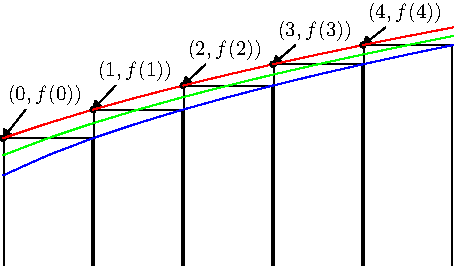
\includegraphics[width=1.00\linewidth]{graphics/intmid.pdf}
\end{center}
\caption{\label{fig:intmid}Comparing sum (black rectangles) with integrals of increasing $f$ (red), $f$ shifted -1/2 (green), and $f$ shifted -1 (blue).}
\label{fig:intmid}
\end{figure}

Summing is a linear operation, so

\begin{equation}
  \sum_{k=0}^{n-1} \left[ \alpha f(k) + \beta g(k) \right] = \alpha \sum_{k=0}^{n-1} f(k) + \beta \sum_{k=0}^{n-1} g(k) \,.
\end{equation}

Summing powers of $k$:

\begin{equation}
  \sum_{k=0}^{n-1} 1 = n \,.
\end{equation}

\begin{equation}
  \sum_{k=0}^{n-1} k = \frac{1}{2} n(n-1) = \frac{1}{2} n^2 + O(n)\,.
\end{equation}

\begin{equation}
  \sum_{k=0}^{n-1} k^2 = \frac{1}{3}n(n-1/2)(n-1) = \frac{1}{3} n^3 + O(n^2) \,.
\end{equation}

\begin{equation}
  \sum_{k=0}^{n-1} k^3 = \frac{1}{4}n^2(n-1)^2 = \frac{1}{4} n^4 + O(n^3) \,.
\end{equation}

Generally, for $p>0$,

\begin{equation}
  \sum_{k=0}^{n-1} k^p \approx \frac{1}{p+1} (n-1/2)^{p+1} = \frac{1}{p+1} n^{p+1} +O(n^p) \,.
\end{equation}

Estimating sums with integrals.

If $f(x)$ is increasing, then
\begin{equation}
\int_{a-1}^{b} f(x) \, dx \leq \sum_{k=a}^{b} f(k) \approx \int_{a-1/2}^{b+1/2} f(x) dx \leq \int_{a}^{b+1} f(x) \, dx
\end{equation}

\end{document}
